% !TeX encoding = utf-8
% !TeX program = pdflatex

\documentclass{CVM}

\usepackage{placeins}

\newcommand{\blu}[1]{\textcolor{blue}{#1}}

% Keep float-only pages compact and top-aligned, including double-column floats.
\makeatletter
\setlength{\@fptop}{0pt}
\setlength{\@fpsep}{14pt}
\setlength{\@fpbot}{0pt plus 1fil}
\setlength{\@dblfptop}{0pt}
\setlength{\@dblfpsep}{14pt}
\setlength{\@dblfpbot}{0pt plus 1fil}
\makeatother

\CVMsetup{
% -- type
type      = {Research Article},
% -- doi
doi       = {CVM.XXXX},
% -- title
title     = {Baseline-Relative Candidate Selection for Training-Free Personalized Segmentation},
% -- author
author    = {First Author$^{1}$\cor{}, Second Author$^{1}$, and Third Author$^{2}$},
% -- runauthor
runauthor = {F. Author, S. Author, T. Author},
% -- abstract
abstract  = {
  Training-free personalized segmentation produces multiple candidate masks, but the query annotation is unavailable when the system must choose one. We study this selection problem in PR-MaGIC and introduce Guarded PR-MaGIC, a baseline-relative fallback policy. The original selector proposes a refinement using support consistency, decoder confidence, and foreground--background separation. The support--foreground gate accepts that proposal only when two internal margins are at least as large as their baseline values. Otherwise, it returns the unrefined mask. Because baseline fallback structurally cannot reduce the non-degradation rate (NDR), an NDR increase alone does not show that the gate is informative. Under rejection-rate matching, guarded mIoU exceeds random fallback by 0.42--1.17 percentage points across five generator--benchmark combinations. The negative gate margin ranks harmful proposals with AUROC values of 0.543--0.633, indicating weak-to-moderate discrimination. In an episode-disjoint calibration targeting 40\% conditional degradation risk, held-out risk remains within the target on FSS-1000 and COCO-20i (35.4--39.9\%) but exceeds it on Pascal-5i (48.0--50.8\%). The policy preserves COCO-20i mIoU and largely removes the original selector's Pascal-5i loss, although accepted refinements can still carry high risk at the default threshold. Transfer to Matcher requires no retraining. These results support conservative candidate replacement while making the limits of the internal risk signals explicit.
},
% -- keywords
keywords  = {personalized segmentation; few-shot segmentation; Segment Anything; training-free inference; iterative refinement; selective prediction},
% -- copyright
copyright = {The Author(s)},
}

%% -- address,

% 1
\address{School of Information and Electrical Engineering, Hunan University of Science and Technology, Xiangtan, Hunan 411201, China. E-mail: 25010401110@mail.hnust.edu.cn.}

% 2
\address{Department or School, Institution Name, City, Postcode, Country. E-mail: authorB@email.edu.}

\begin{document}

\maketitle

\begin{figure}[t]
\centering
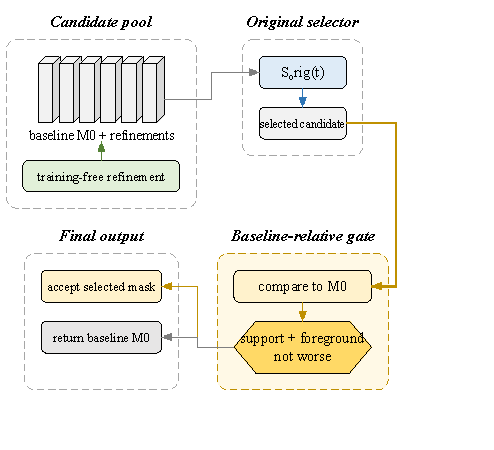
\includegraphics[width=\linewidth]{figures/generated/cvpr_guarded_prmagic_graphical_abstract.pdf}
\caption{Overview of Guarded PR-MaGIC. The candidate pool contains a baseline mask $M_0$ and refined candidates $M_1,\ldots,M_T$. The original selector proposes a candidate, and the baseline-relative support--foreground gate either accepts it or falls back to $M_0$. The framework works with PerSAM-F and Matcher candidate generators and uses no query ground truth during inference.}
\label{fig:overview}
\end{figure}

\section{Introduction}

Visual foundation models have changed how segmentation systems are built. The Segment Anything Model (SAM) provides a promptable mask decoder that generalizes across diverse images. Personalized and few-shot methods extend this setting by transferring a target concept from a reference image and mask to a query image. This training-free setup is especially useful when annotations or computation are limited.

The main unresolved problem appears after candidate generation. Iterative refinement can produce masks of very different quality, but the query annotation is unavailable at deployment. The system must therefore choose a mask using internal signals alone. Average mIoU can hide this decision risk: a selector may improve the mean while degrading many episodes. The problem is particularly acute in one-shot segmentation, where a single reference image may not resolve background interference, appearance changes, or object ambiguity.

We study this problem in a training-free iterative segmentation pipeline based on PR-MaGIC~\cite{12}. The pipeline updates the query representation along a direction derived from the SAM mask decoder and produces one candidate at each refinement step. The original selector combines support--query similarity, decoder confidence, and foreground--background separation. Its behavior depends on the benchmark: it improves mean mIoU on FSS-1000 and COCO-20i but reduces it on Pascal-5i by 1.75 percentage points. In all three benchmarks, the oracle candidate outperforms the selected result. This gap separates the quality of the candidate pool from the quality of the selection rule.

We therefore introduce a baseline-relative selection layer, the support--foreground gate. It accepts the original proposal only when two complementary signals are no worse than their baseline values. Otherwise, it returns candidate 0. The baseline serves as the reference action in a selective prediction policy. The gate is training-free, uses no query ground truth, and operates online after candidate generation.

Figure~\ref{fig:overview} summarizes the separation between candidate generation, ranking, and baseline-relative acceptance. The architecture leaves candidate generation unchanged and applies the selection rule only at the final decision stage.

The contributions are:

\begin{enumerate}
\item We frame candidate selection in training-free iterative segmentation as a selective prediction problem and derive the structural NDR property induced by baseline fallback.
\item We introduce a baseline-relative support--foreground gate for conservative candidate replacement.
\item We evaluate gate informativeness with rejection-rate-matched random fallback, proposal-level discrimination, paired analyses, and risk--coverage curves.
\item We transfer the gate to the independent Matcher candidate generator on FSS-1000 and COCO-20i.
\item We test an episode-disjoint calibration protocol, including both its successes on FSS-1000 and COCO-20i and its failure on Pascal-5i.
\end{enumerate}

\section{Related Work}

\subsection{Promptable and Personalized Segmentation}

SAM introduced promptable segmentation with a large-scale image encoder, a prompt encoder, and a mask decoder~\cite{1}. PerSAM adapts this paradigm to personalized segmentation by extracting a target concept from a reference image and mask. PerSAM-F adds an efficient fine-tuning variant with few learnable parameters~\cite{2}. We use a PerSAM-F-compatible pipeline as one candidate generator, but focus on the separate problem of choosing among iterative candidates without query labels.

\subsection{Few-Shot and In-Context Segmentation}

Few-shot semantic segmentation represents an episode with support images, support masks, and a query image. Prototype alignment, hypercorrelation, and related methods transfer support information to query pixels~\cite{3,4,5}. Painter and SegGPT study visual in-context prediction with foundation-model representations~\cite{6,7}. These methods establish the value of reference information, but standard evaluation mainly reports mean segmentation quality. We add a candidate-level analysis of non-degradation and selection reliability.

\subsection{SAM-Based Reference Matching}

Matcher performs one-shot segmentation by matching support and query features, then using the correspondences to construct SAM prompts~\cite{8}. VRP-SAM introduces a visual reference prompt encoder and evaluates point, scribble, box, and mask prompts for one-shot semantic segmentation~\cite{9}. These methods provide external performance context. Our contribution addresses a different stage: a baseline-relative selection layer that operates after a candidate generator has produced multiple masks.

\subsection{Selective Prediction and Risk Control}

Selective prediction augments a predictor with a reject option and studies the trade-off between coverage and conditional risk~\cite{13}. The framework has been extended to deep neural networks, where confidence-based rejection can target a prescribed risk level~\cite{14}. Distribution-free risk-controlling prediction sets instead use held-out calibration data to obtain finite-sample guarantees~\cite{15}. We adopt the reject-option perspective, but we do not claim calibrated or distribution-free risk control. Our method is a heuristic baseline-relative policy whose informativeness must be tested empirically under rejection-rate matching.

\section{Problem Formulation}

Let $I_s$ and $Y_s$ denote a support image and its reference mask, and let $I_q$ denote a query image. A training-free personalized segmentation system produces a baseline mask $M_0$ and refined candidates $M_1,\ldots,M_T$. The candidate set is
\begin{align}
\mathcal{M}=\{M_0,M_1,\ldots,M_T\}.
\label{eq:candidates}
\end{align}
The query ground truth $Y_q$ is unavailable during inference and is used only for evaluation. A selector receives internal diagnostics $\mathbf{q}(t)$ for each candidate and returns an index $\hat{t}$. The deployed output is $M_{\hat{t}}$. Each episode contains one foreground target, so its score is an IoU. We use mIoU for the mean of episode-level IoUs across an evaluation set.

For analysis, we define the non-degradation rate (NDR) as
\begin{align}
\mathrm{NDR}=\frac{1}{N}\sum_{i=1}^{N}
\mathbb{1}\left[
\mathrm{IoU}(M_{\hat{t}_i},Y_{q,i})
\geq
\mathrm{IoU}(M_{0,i},Y_{q,i})
\right].
\label{eq:ndr}
\end{align}
Unlike mIoU, NDR records whether a policy replaces the baseline with a worse prediction on an episode. It describes output behavior relative to the baseline, but it does not measure whether the gate can identify harmful proposals.

\subsection{Selective Prediction View}

The guarded selector is a selective prediction policy over neural candidates. Let $p_i=\mathbb{1}[t_i^*\neq 0]$ indicate a non-baseline proposal, and let $a_i=\mathbb{1}[\hat{t}_i\neq 0]$ indicate an accepted refinement. We define refinement coverage, total baseline output, and gate-triggered fallback as
\begin{align}
\mathrm{Coverage}&=\frac{1}{N}\sum_{i=1}^{N}a_i,\\
\mathrm{BaselineOutput}&=1-\mathrm{Coverage},\\
\mathrm{GateFallback}&=\frac{1}{N}\sum_{i=1}^{N}(p_i-a_i).
\label{eq:coverage}
\end{align}
Let
\begin{align}
d_i=\mathbb{1}\left[
\mathrm{IoU}(M_{t_i^*},Y_{q,i})<\mathrm{IoU}(M_{0,i},Y_{q,i})
\right]
\label{eq:proposal_degradation}
\end{align}
indicate that the original proposal is worse than the baseline. Because a rejected proposal is replaced by $M_0$, the guarded NDR satisfies
\begin{align}
\mathrm{NDR}_{\mathrm{guarded}}
=\mathrm{NDR}_{\mathrm{original}}
+\frac{1}{N}\sum_{i=1}^{N}(p_i-a_i)d_i
\geq \mathrm{NDR}_{\mathrm{original}}.
\label{eq:ndr_monotonicity}
\end{align}
This inequality is structural for any baseline-fallback rule, including random rejection. An all-fallback policy would attain 100\% NDR while providing no refinement utility. We therefore evaluate gate informativeness using mIoU retention, rejection-rate-matched random fallback, and proposal-level discrimination.

For analysis only, define the baseline-relative loss of an accepted decision as
\begin{align}
\ell_i=\left[\mathrm{IoU}(M_{0,i},Y_{q,i})-\mathrm{IoU}(M_{\hat{t}_i},Y_{q,i})\right]_+.
\label{eq:selective_loss}
\end{align}
The conditional selective risk is the mean of $\ell_i$ over accepted refinements. The policy does not use $Y_q$, but Eqs.~\eqref{eq:coverage} and~\eqref{eq:selective_loss} evaluate the cost of acceptance retrospectively. We report NDR together with mIoU and coverage rather than treating it as standalone evidence of signal quality. BaselineOutput measures total abstention, whereas GateFallback measures proposals actively rejected by the gate.

\section{Method}

\subsection{Training-Free Candidate Generation}

We use a PR-MaGIC-style generator~\cite{12} built on a PerSAM-F-compatible personalized SAM pipeline. We encode the support image and use its masked features to define the target concept. Personalized points are sampled from the similarity map, and the mask decoder then produces the baseline candidate. At each refinement step, a decoder-gradient direction updates the query feature space. If $F_q^{(t)}$ denotes the query representation at iteration $t$, the update is
\begin{align}
F_q^{(t+1)}=F_q^{(t)}+\eta V^{(t)}+\sqrt{2\eta\gamma}\,\epsilon^{(t)},
\label{eq:update}
\end{align}
where $V^{(t)}$ is a clipped decoder-gradient direction and $\eta$ is the step size. The random variable $\epsilon^{(t)}\sim\mathcal{N}(0,I)$ supplies Gaussian perturbations, while $\gamma$ controls their variance. We use six candidates in the reported experiments: one baseline and five refinements.

Figure~\ref{fig:detailed_framework} shows the complete inference pipeline. Reference-conditioned features generate the candidate pool, the original score ranks the candidates, and the gate determines whether the selected refinement replaces $M_0$.

\begin{figure}[t]
\centering
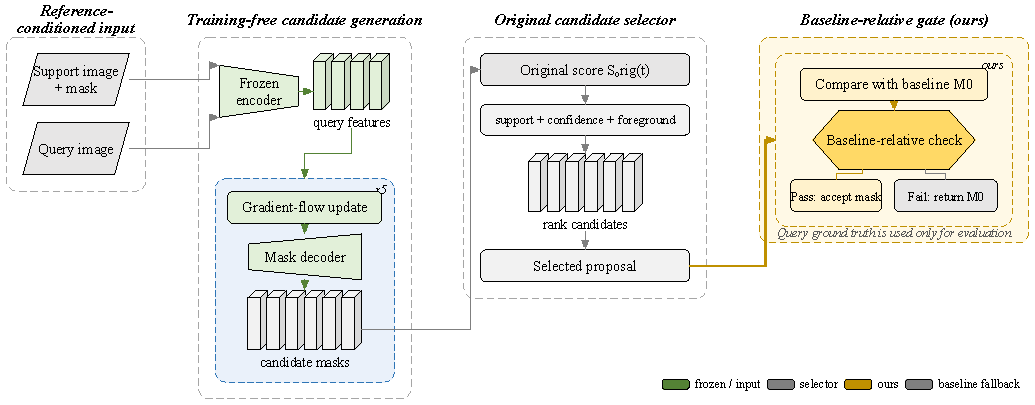
\includegraphics[width=\linewidth]{figures/generated/cvpr_guarded_prmagic_framework.pdf}
\caption{Detailed schematic of Guarded PR-MaGIC. A support image, support mask, and query image define a reference-conditioned episode. Frozen representations and mask-decoder gradient flow generate a candidate set $\{M_0,\ldots,M_T\}$. The original selector proposes $t^*$, after which the baseline-relative support--foreground gate either accepts $M_{t^*}$ or returns to the unrefined baseline $M_0$. The query ground truth is used only for evaluation.}
\label{fig:detailed_framework}
\end{figure}

\subsection{Original Candidate Selector}

For each candidate, we compute four diagnostics: support--query consistency $q_{\mathrm{sup}}(t)$, decoder confidence $q_{\mathrm{dec}}(t)$, temporal stability $q_{\mathrm{tmp}}(t)$, and foreground--background separation $q_{\mathrm{fg}}(t)$. The original selector combines three of them as
\begin{align}
S_{\mathrm{orig}}(t)=q_{\mathrm{sup}}(t)+\alpha q_{\mathrm{dec}}(t)+\beta q_{\mathrm{fg}}(t),
\label{eq:original}
\end{align}
where $\alpha=0.25$ and $\beta=0.10$. It proposes
\begin{align}
t^*=\arg\max_{t\in\{0,\ldots,T\}}S_{\mathrm{orig}}(t).
\label{eq:proposal}
\end{align}
Because $q_{\mathrm{tmp}}$ measures agreement with the preceding candidate rather than quality relative to $M_0$, the original score retains it only as a diagnostic. Section~\ref{sec:gate_ablation} separately tests its use as an additional gate condition.
The original policy outputs $M_{t^*}$ even when the proposal is worse than $M_0$ under the query ground truth.

\subsection{Baseline-Relative Neural Inference}

We separate candidate generation from candidate acceptance. The neural generator maps a support/query episode to an internal state and a candidate set,
\begin{align}
\Phi(I_s,Y_s,I_q)=\left(\mathcal{M},\mathbf{q}(0),\ldots,\mathbf{q}(T)\right),
\label{eq:neural_state}
\end{align}
where $\Phi$ includes frozen encoder features, decoder outputs, and iterative gradient-flow states. The selector is an inference-time policy $\pi$, not a new trainable segmentation network. Baseline-relative selection is applied before the output mask is released, using evidence produced by the generator itself.

This separation has two practical consequences. First, the generator can be improved without changing the selection rule. Second, the same rule can transfer to an independent generator when comparable higher-is-better diagnostics are available. The gate is therefore a selection layer for SAM-based reference segmentation, not a universal score-calibration method.

\subsection{Baseline-Relative Gate}

The gate compares each signal with its baseline value:
\begin{align}
\Delta q_k(t)=q_k(t)-q_k(0).
\label{eq:delta}
\end{align}
For a signal subset $\mathcal{S}$ and tolerances $\tau_k$, we define
\begin{align}
G_{\mathcal{S},\boldsymbol{\tau}}(t^*)=
\mathbb{1}\left[\Delta q_k(t^*)\geq-\tau_k,\ \forall k\in\mathcal{S}\right].
\label{eq:general_gate}
\end{align}
The final index is
\begin{align}
\hat{t}=\begin{cases}
t^*, & G_{\mathcal{S},\boldsymbol{\tau}}(t^*)=1,\\
0, & G_{\mathcal{S},\boldsymbol{\tau}}(t^*)=0.
\end{cases}
\label{eq:guarded}
\end{align}
The formulation separates candidate generation, candidate ranking, and candidate acceptance. It also supports controlled ablations by changing $\mathcal{S}$ while keeping the candidate pool fixed.

\subsection{Support--Foreground Instantiation}

Our default gate, denoted support\_fg, uses
\begin{align}
\mathcal{S}=\{\mathrm{sup},\mathrm{fg}\},\qquad \tau_{\mathrm{sup}}=\tau_{\mathrm{fg}}=0.
\label{eq:supportfg}
\end{align}
It accepts a non-baseline proposal only when its masked support--query consistency and foreground--background separation are no worse than the corresponding baseline values. The gate does not inspect $Y_q$ or alter the generator.

For risk--coverage analysis, we summarize the two baseline-relative margins by
\begin{align}
m_i=\min\left\{
q_{\mathrm{sup},i}(t_i^*)-q_{\mathrm{sup},i}(0),
q_{\mathrm{fg},i}(t_i^*)-q_{\mathrm{fg},i}(0)
\right\},
\label{eq:margin}
\end{align}
for episodes with a non-baseline proposal, $t_i^*\neq 0$. At threshold $\lambda$, the policy accepts the proposal when $m_i\geq\lambda$ and otherwise outputs the baseline. The main experiments use $\lambda=0$. Sweeping $\lambda$ changes the operating point without changing candidate generation or ranking.

\subsection{Implementation and Computational Behavior}

The guarded selector is available through \texttt{--selector guarded}. Because the original selector already computes the required diagnostics, the gate adds only scalar comparisons and requires no training stage. We also replay the gate from candidate-level CSV files for paired comparisons. The mean selected iteration provides an operational measure of how conservatively the policy selects candidates.

\section{Experimental Setup}

\subsection{Benchmarks and Evaluation Protocol}

We evaluate one-shot personalized or in-context segmentation on FSS-1000~\cite{10}, COCO-20i~\cite{11}, and Pascal-5i~\cite{3}. FSS-1000 uses seeds 42--44 with 2,400 episodes per seed. COCO-20i and Pascal-5i use seeds 45--47, folds 0--3, and 1,000 episodes per fold. In total, we evaluate 7,200 FSS-1000 episodes and 12,000 episodes for each of COCO-20i and Pascal-5i.

The PerSAM-F-compatible experiments use one support shot, five prompt points, and six candidates, including the baseline, with $\eta=10^{-3}$, $\gamma=10^{-1}$, $\alpha=0.25$, and $\beta=0.10$. The Matcher transfer experiments use one shot, six nested candidates, $\mathrm{points\_per\_side}=32$, $\mathrm{points\_per\_batch}=16$, eight centers, and five merged masks. Both configurations run with SAM ViT-H and DINOv2 ViT-L/14 on 24-GB GPUs. The original and guarded policies use identical settings. Table~\ref{tab:protocol} summarizes the protocol.

\begin{table*}[h!t]
\center
\caption{Evaluation protocol used in this study.}
\begin{tabular}{llllll}
\toprule
Benchmark & Setting & Folds & Seeds & Episodes & Candidate generator \\
\midrule
FSS-1000 & one-shot & fold 0 & 42, 43, 44 & 2,400/seed & PerSAM-F-compatible \\
COCO-20i & one-shot & 0--3 & 45, 46, 47 & 1,000/fold & PerSAM-F-compatible \\
Pascal-5i & one-shot & 0--3 & 45, 46, 47 & 1,000/fold & PerSAM-F-compatible \\
FSS-1000 & one-shot & fold 0 & 42 & 2,400 & Matcher \\
COCO-20i & one-shot & fold 0 & 42 & 1,000 & Matcher \\
\bottomrule
\end{tabular}
\label{tab:protocol}
\end{table*}

\subsection{Compared Policies and Statistics}

We compare the baseline, original selector, confidence-only, support-only, foreground-only, and support\_fg policies. The oracle selects the best candidate using query ground truth and serves only as an upper bound. The episode is the independent resampling unit. Paired policy differences use 10,000 episode-level bootstrap resamples and percentile 95\% intervals.

We also compare support\_fg with a rejection-rate-matched random fallback policy. Within each generator--benchmark group, this control samples non-baseline proposals without replacement and rejects exactly as many as support\_fg. We repeat the random assignment 10,000 times with seed 20260907 and report 95\% randomization intervals. These intervals describe random policy assignments on the fixed evaluation set, not population-level sampling uncertainty.

We evaluate proposal-level discrimination only for non-baseline proposals. We use $-m_i$ as the risk score and $d_i$ from Eq.~\eqref{eq:proposal_degradation} as the binary outcome. We report AUROC, average precision (AP), rejection precision, and conditional degradation risk among accepted refinements. AUROC and AP intervals use 2,000 episode-level bootstrap resamples with seed 20260907. Discrimination is computed on all non-baseline proposals with defined margins; episodes whose original proposal is the baseline are excluded from this analysis only.

We also test an empirical episode-disjoint calibration protocol with a target conditional degradation risk of $\epsilon=0.40$. For each benchmark, a deterministic hash of the episode identifier reserves approximately 20\% of episodes from the first seed for calibration and holds out the remainder. The first seed is 42 for FSS-1000 and 45 for COCO-20i and Pascal-5i. We choose the highest-coverage threshold $\lambda$ whose empirical calibration risk is at most $\epsilon$. We then fix that threshold for the held-out episodes from the calibration seed and the matching held-out episode identifiers from the other two seeds. Query annotations are used offline to select $\lambda$. This analysis therefore does not turn the default $\lambda=0$ gate into a calibrated or distribution-free procedure. Instead, it provides an episode-disjoint stress test of threshold transfer.

\subsection{External Published Results}

Published results from PerSAM/PerSAM-F~\cite{2}, Matcher~\cite{8}, and VRP-SAM~\cite{9} provide external context. We did not rerun these methods under our protocol. Their reported results use different encoders, prompt formats, fold aggregations, and, in some cases, benchmark subsets. We therefore treat these values as contextual comparisons.

\section{Results}

\subsection{Candidate-Selection Instability}

We first quantify instability in the unguarded policy. Table~\ref{tab:instability} reports the baseline, selected result, oracle result, degradation rate, and selector regret, defined as oracle mIoU minus selected mIoU. On Pascal-5i, the original policy degrades 61.43\% of episodes and leaves a regret of 0.099298, even though the candidate pool contains a much stronger oracle. Candidate generation and candidate selection therefore need to be evaluated separately.

\begin{table*}[h!t]
\center
\caption{Instability of the unguarded selector. Degradation rate is $1-\mathrm{NDR}$, and selector regret is oracle mIoU minus selected mIoU.}
\begin{tabular}{llrrrrr}
\toprule
Generator & Benchmark & Baseline & Original & Oracle & Degradation & Regret \\
\midrule
PerSAM-F-compatible & FSS-1000 & 0.857831 & 0.885044 & 0.918510 & 36.68\% & 0.033466 \\
PerSAM-F-compatible & COCO-20i & 0.535171 & 0.565638 & 0.638627 & 33.22\% & 0.072990 \\
PerSAM-F-compatible & Pascal-5i & 0.669651 & 0.652193 & 0.751492 & 61.43\% & 0.099298 \\
Matcher & FSS-1000 & 0.884484 & 0.903832 & 0.923176 & 35.00\% & 0.019344 \\
Matcher & COCO-20i & 0.681014 & 0.698208 & 0.736494 & 33.20\% & 0.038286 \\
\bottomrule
\end{tabular}
\label{tab:instability}
\end{table*}

Degradation occurs with both candidate generators and across benchmark families. This pattern motivates Eq.~\eqref{eq:guarded}: the system should fall back when its internal evidence is less favorable than the baseline.

Figure~\ref{fig:instability_visual} shows one high-regret episode from each PerSAM-F-compatible benchmark. The blue curve shows candidate mIoU, and the orange curve shows the normalized selector score. The original proposal differs from the oracle candidate in all three examples. These cases are illustrative; aggregate claims use the complete paired evaluations.

\begin{figure*}[t]
\centering
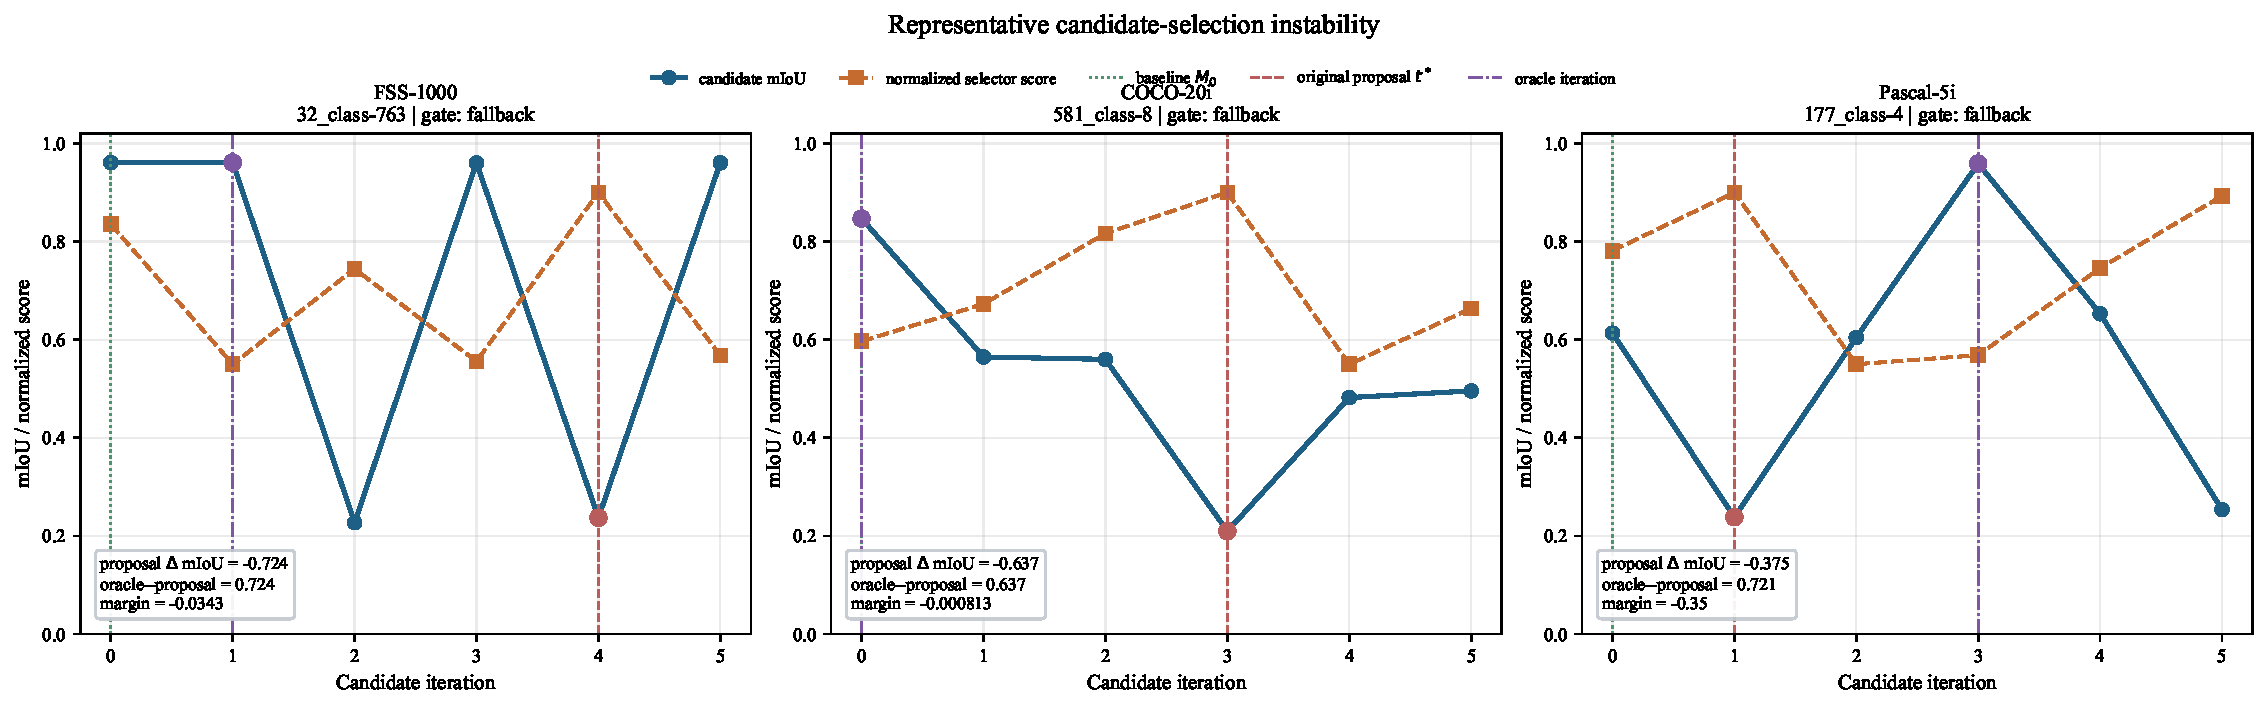
\includegraphics[width=.98\linewidth]{figures/generated/candidate_instability.pdf}
\caption{Representative candidate-selection instability reconstructed from the saved candidate CSVs. The blue curve shows candidate mIoU, and the orange dashed curve shows the original selector score after within-episode normalization. Green, red, and purple vertical markers identify the baseline, original proposal, and oracle candidate, respectively. Each episode is a high-regret illustration; query mIoU is used only for retrospective annotation and is unavailable to the selector and gate.}
\label{fig:instability_visual}
\end{figure*}

\subsection{Main Cross-Benchmark Results}

Table~\ref{tab:main} reports the PerSAM-F-compatible results. The original selector improves mIoU on FSS-1000 and COCO-20i but loses mIoU on Pascal-5i. The support\_fg gate preserves COCO-20i mIoU and brings Pascal-5i within 0.05 percentage points of the baseline. NDR rises on all three benchmarks, as expected from the baseline-fallback construction in Eq.~\eqref{eq:ndr_monotonicity}.

Figure~\ref{fig:benchmark_summary} summarizes these comparisons. The mIoU effect remains benchmark-dependent despite the structural NDR increase. Guarded selection trades some FSS-1000 mIoU for fewer degradations, preserves COCO-20i quality, and recovers most of the original selector's Pascal-5i loss. The fallback panel shows how often the policy returns to the baseline.

\begin{figure*}[t]
\centering
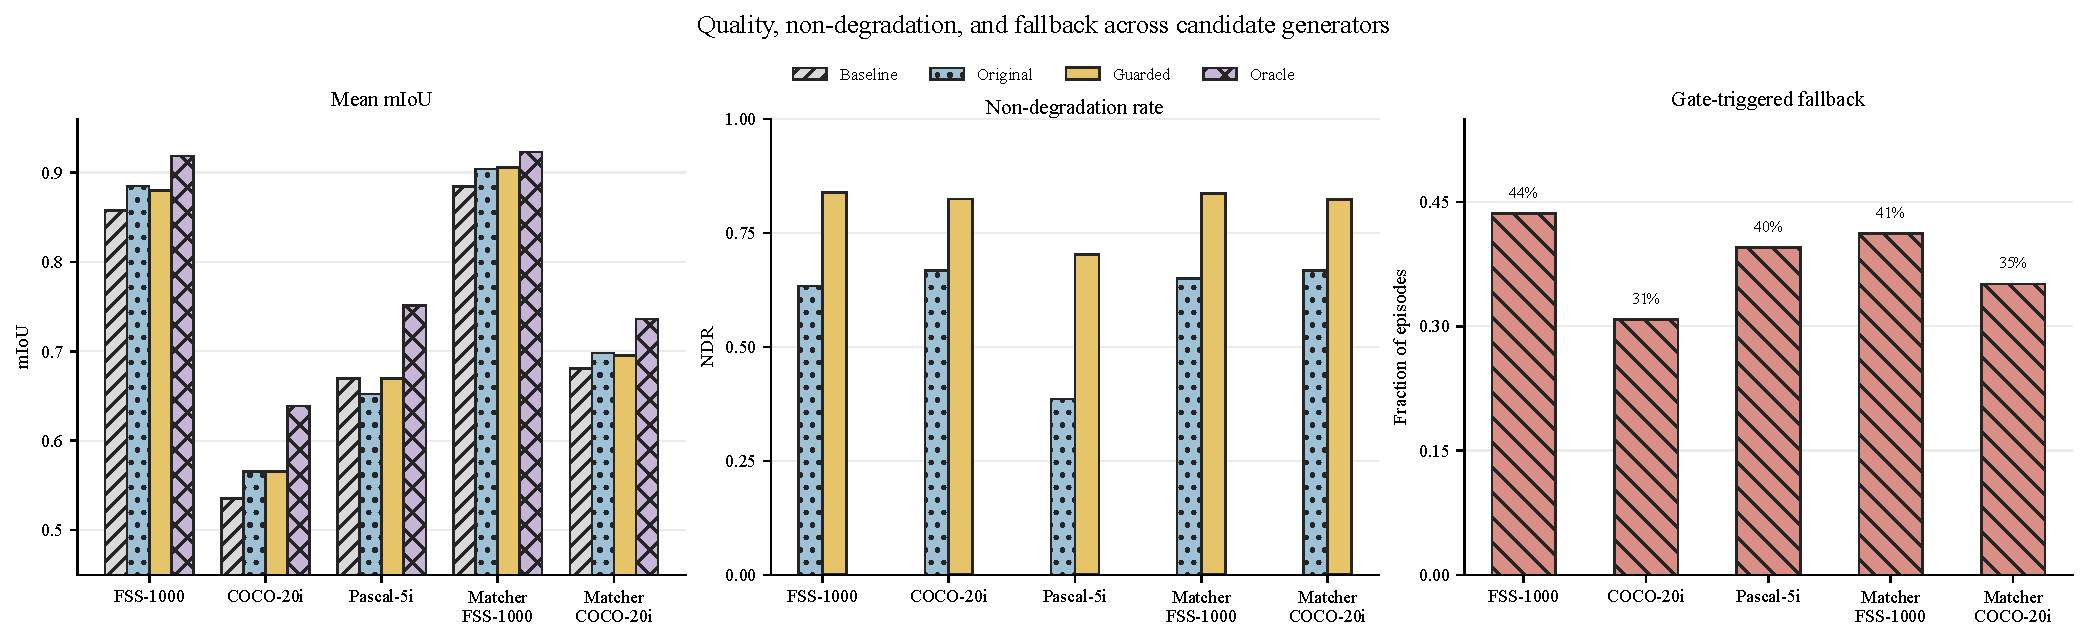
\includegraphics[width=\linewidth]{figures/generated/benchmark_summary.pdf}
\caption{Quality, baseline-relative non-degradation, and fallback behavior of the guarded selector. Left: mIoU for the baseline, original selector, guarded selector, and candidate-pool oracle. Center: non-degradation rate (NDR), whose monotonic increase follows from baseline fallback. Right: fraction of non-baseline proposals rejected by the gate. Matcher rows show independent-generator transfer experiments. Hatching preserves the comparison in grayscale.}
\label{fig:benchmark_summary}
\end{figure*}

\begin{table*}[h!t]
\center
\caption{PerSAM-F-compatible results over the saved full evaluation sets. mIoU is reported as an absolute value, and gains are percentage-point differences. Guarded denotes the support\_fg gate. Gate fallback counts non-baseline proposals rejected by the gate; it excludes episodes for which the original selector already chooses candidate 0.}
\begin{tabular}{lrrrrrr}
\toprule
Benchmark & Baseline & Original & Guarded & Original NDR & Guarded NDR & Gate fallback \\
\midrule
FSS-1000 & 0.857831 & 0.885044 & 0.879513 & 63.32\% & 83.81\% & 43.61\% \\
COCO-20i & 0.535171 & 0.565638 & 0.565979 & 66.78\% & 82.43\% & 30.78\% \\
Pascal-5i & 0.669651 & 0.652193 & 0.669199 & 38.58\% & 70.22\% & 39.50\% \\
\bottomrule
\end{tabular}
\label{tab:main}
\end{table*}

On FSS-1000, the original selector gains 2.721 percentage points over the baseline. The gate gives up 0.553 points relative to the original selector in exchange for a 20.49-point NDR increase. On COCO-20i, guarded mIoU is 0.565979 versus 0.565638 for the original selector, while NDR rises by 15.64 points. On Pascal-5i, the original selector is 1.746 points below the baseline, whereas support\_fg is only 0.045 points below it and improves on the original selector by 1.701 points.

The three-seed analysis shows the same pattern at the benchmark level. On COCO-20i, the original selector gains 3.047, 3.045, and 2.988 percentage points over the baseline for seeds 45, 46, and 47, respectively. The guarded selector gains 3.081, 3.087, and 3.045 points. On Pascal-5i, the original selector remains below the baseline for all three seeds, whereas the guarded selector stays within 0.10 percentage points of the baseline for every seed. The gate is therefore best viewed as a baseline-relative selection policy with a benchmark-dependent quality--safety operating point.

\subsection{Gate Informativeness under Rejection-Rate Matching}

NDR cannot distinguish an informative gate from indiscriminate fallback because both policies replace rejected proposals with the baseline. We therefore compare support\_fg with random fallback under rejection-rate matching. Table~\ref{tab:random_control} reports the randomization distribution for each fixed evaluation set.

\begin{table*}[h!t]
\center
\caption{Rejection-rate-matched random fallback control. Random fallback rejects the same number of non-baseline proposals as support\_fg in each group. Brackets show 95\% randomization intervals over 10,000 assignments. The final column reports the guarded-minus-random mIoU difference in percentage points.}
\begin{tabular}{llrrrr}
\toprule
Generator & Benchmark & Fallback & Random mIoU & Guarded mIoU & Difference [95\% RI] \\
\midrule
PerSAM-F-compatible & FSS-1000 & 43.61\% & 0.870853 [0.869070, 0.872677] & 0.879513 & +0.866 [0.684, 1.044] pp \\
PerSAM-F-compatible & COCO-20i & 30.78\% & 0.554368 [0.552988, 0.555747] & 0.565979 & +1.161 [1.023, 1.299] pp \\
PerSAM-F-compatible & Pascal-5i & 39.50\% & 0.660441 [0.658815, 0.662076] & 0.669199 & +0.876 [0.712, 1.038] pp \\
Matcher & FSS-1000 & 41.17\% & 0.894231 [0.891718, 0.896733] & 0.905907 & +1.168 [0.917, 1.419] pp \\
Matcher & COCO-20i & 35.10\% & 0.690729 [0.687697, 0.693800] & 0.694956 & +0.423 [0.116, 0.726] pp \\
\bottomrule
\end{tabular}
\label{tab:random_control}
\end{table*}

Guarded mIoU exceeds random fallback in all five comparisons by 0.42--1.17 percentage points. Every guarded-minus-random interval is positive, with lower bounds of 0.12--1.02 points. Thus, at the same abstention level, the gate retains more segmentation quality than indiscriminate fallback.

We next ask whether the gate margin ranks harmful proposals above non-harmful ones. Table~\ref{tab:discrimination} reports proposal-level discrimination using $-m_i$ as the risk score. AUROC ranges from 0.543 to 0.633, indicating weak-to-moderate ranking ability rather than calibrated risk estimation.

\begin{table*}[h!t]
\center
\caption{Proposal-level discrimination of the baseline-relative gate margin. AUROC and average precision (AP) use proposal degradation as the positive outcome. Brackets show percentile 95\% intervals from 2,000 episode-level bootstrap resamples. Rejection precision is the fraction of rejected proposals that are degraded. Accepted risk is the fraction of accepted non-baseline proposals that are degraded.}
\begin{tabular}{llrrrr}
\toprule
Generator & Benchmark & AUROC & AP & Rejection precision & Accepted risk \\
\midrule
PerSAM-F-compatible & FSS-1000 & 0.543 [0.529, 0.558] & 0.452 [0.435, 0.470] & 46.97\% & 40.46\% \\
PerSAM-F-compatible & COCO-20i & 0.629 [0.618, 0.640] & 0.488 [0.474, 0.505] & 50.81\% & 33.52\% \\
PerSAM-F-compatible & Pascal-5i & 0.633 [0.618, 0.648] & 0.761 [0.749, 0.773] & 80.11\% & 67.63\% \\
Matcher & FSS-1000 & 0.575 [0.549, 0.601] & 0.484 [0.451, 0.519] & 45.45\% & 38.79\% \\
Matcher & COCO-20i & 0.545 [0.505, 0.583] & 0.425 [0.380, 0.475] & 44.44\% & 38.68\% \\
\bottomrule
\end{tabular}
\label{tab:discrimination}
\end{table*}

Pascal-5i exposes the main limitation. Rejected proposals are enriched for degradation, with 80.11\% rejection precision, but 67.63\% of accepted refinements still fall below the baseline. The Pascal-5i NDR increase therefore comes mainly from frequent fallback rather than precise identification of safe refinements.

\subsection{Paired Statistical Analysis}

On COCO-20i, support\_fg differs from the original selector by $+0.000341$ mIoU, with a 95\% interval of $[-0.001045,+0.001700]$. This interval is consistent with preserved average quality. The corresponding 15.64-point NDR increase quantifies the effect of fallback, but it does not independently test gate discrimination.

On Pascal-5i, support\_fg improves mIoU by $+0.017006$, with a 95\% interval of $[+0.015167,+0.018918]$. NDR rises by 31.64 percentage points, with an interval of $[+30.80,+32.48]$. No episode becomes newly degraded because the policy either preserves the original proposal or returns to the baseline.

On FSS-1000, support\_fg raises NDR by 20.49 percentage points but lowers mIoU by 0.553 points relative to the original selector. The mIoU interval is $[-0.722,-0.391]$ points, whereas the NDR interval is $[+19.51,+21.43]$ points. The trade-off is clear: a conservative gate can reject useful candidates as well as risky ones.

\subsection{Gate Ablation}
\label{sec:gate_ablation}

Table~\ref{tab:ablation} reports the gate ablation. The confidence-only variant shows why a single decoder score is not enough: it raises NDR through additional fallback but loses mIoU on FSS-1000 and COCO-20i. The support--foreground gate gives the best mIoU on Pascal-5i and the highest NDR among the tested variants.

\begin{table*}[h!t]
\center
\caption{Gate ablation over the complete saved benchmark groups. Each benchmark uses the same candidate pool for all policies. Gate fallback counts non-baseline proposals actively rejected by the corresponding gate.}
\begin{tabular}{llrrrr}
\toprule
Benchmark & Policy & mIoU & Gain over baseline & NDR & Gate fallback \\
\midrule
FSS-1000 & Original & 0.885044 & +2.721 pp & 63.32\% & 0.00\% \\
FSS-1000 & Confidence only & 0.876292 & +1.846 pp & 69.28\% & 13.93\% \\
FSS-1000 & Support only & 0.882009 & +2.418 pp & 75.21\% & 25.44\% \\
FSS-1000 & Foreground only & 0.882666 & +2.484 pp & 74.26\% & 22.32\% \\
FSS-1000 & \textbf{Support + foreground} & \textbf{0.879513} & +2.168 pp & \textbf{83.81\%} & 43.61\% \\
\midrule
COCO-20i & Original & 0.565638 & +3.047 pp & 66.78\% & 0.00\% \\
COCO-20i & Confidence only & 0.559263 & +2.409 pp & 71.95\% & 14.46\% \\
COCO-20i & Support only & 0.565497 & +3.033 pp & 77.09\% & 19.56\% \\
COCO-20i & Foreground only & 0.566304 & +3.113 pp & 73.25\% & 13.23\% \\
COCO-20i & \textbf{Support + foreground} & \textbf{0.565979} & +3.081 pp & \textbf{82.43\%} & 30.78\% \\
\midrule
Pascal-5i & Original & 0.652193 & -1.746 pp & 38.58\% & 0.00\% \\
Pascal-5i & Confidence only & 0.659334 & -1.032 pp & 49.78\% & 15.68\% \\
Pascal-5i & Support only & 0.657808 & -1.184 pp & 57.33\% & 23.62\% \\
Pascal-5i & Foreground only & 0.664418 & -0.523 pp & 53.60\% & 18.18\% \\
Pascal-5i & \textbf{Support + foreground} & \textbf{0.669199} & -0.045 pp & \textbf{70.22\%} & 39.50\% \\
\bottomrule
\end{tabular}
\label{tab:ablation}
\end{table*}

The ablation shows that the two gate signals produce different quality--fallback trade-offs. Foreground-only gives the highest COCO-20i mIoU among the gated variants, whereas support\_fg rejects more proposals. We therefore use support\_fg as a conservative operating point, not as a universal mIoU maximizer. NDR comparisons across gates should be read alongside their different fallback rates.

We also tested temporal stability as a third acceptance condition. Because candidate 0 has temporal stability 1 by construction, the literal baseline-relative rule accepted no refinements on the PerSAM-F-compatible FSS-1000 or COCO-20i evaluations and only 1 of 12,000 on Pascal-5i. Among proposals already accepted by support\_fg, temporal deficit ranked degraded proposals below chance in all five generator--benchmark evaluations (AUROC 0.269--0.456). We therefore exclude this local stability signal from the default gate.

\subsection{Transfer to the Matcher Candidate Generator}

We then test whether the gate depends on the PerSAM-F implementation. Matcher is an independent SAM-based feature-matching pipeline. We apply the same policies to identical candidate pools on FSS-1000 and COCO-20i. Table~\ref{tab:matcher} reports the results.

\begin{table*}[h!t]
\center
\caption{Transfer experiment using the independent Matcher candidate generator.}
\begin{tabular}{lrrrrrr}
\toprule
Benchmark & Baseline & Original & Guarded & Original NDR & Guarded NDR & NDR gain \\
\midrule
FSS-1000 & 0.884484 & 0.903832 & 0.905907 & 65.00\% & 83.71\% & +18.71 pp \\
COCO-20i & 0.681014 & 0.698208 & 0.694956 & 66.80\% & 82.40\% & +15.60 pp \\
\bottomrule
\end{tabular}
\label{tab:matcher}
\end{table*}

The paired Matcher analysis contains 2,400 FSS-1000 episodes and 1,000 COCO-20i episodes. On FSS-1000, guarding changes mIoU by $+0.002075$; on COCO-20i, it changes mIoU by $-0.003252$. Across 3,400 episodes, the pooled difference is $+0.000508$, with a 95\% interval of $[-0.001317,+0.002366]$. Rejection-rate-matched controls remain favorable on both benchmarks, exceeding random fallback by 1.168 and 0.423 percentage points, respectively. The rule therefore transfers without retraining, although the margin remains a weak discriminator in these Matcher experiments.

\subsection{Risk--Coverage Behavior}

To make the selective-prediction interpretation explicit, we sweep the margin in Eq.~\eqref{eq:margin}. For each threshold, we report accepted-refinement coverage and conditional degradation risk,
\begin{align}
\mathrm{Risk}_{\mathrm{deg}}(\lambda)=
\frac{\sum_{i=1}^{N}a_i(\lambda)\,\mathbb{1}\left[
\mathrm{IoU}(M_{t_i^*},Y_{q,i})<\mathrm{IoU}(M_{0,i},Y_{q,i})
\right]}
{\sum_{i=1}^{N}a_i(\lambda)},
\label{eq:riskcoverage}
\end{align}
where $a_i(\lambda)=1$ only when the proposal is non-baseline and its margin is at least $\lambda$. Query annotations are used only for retrospective evaluation. We use degradation risk as the primary y-axis because it directly captures the harm that NDR is designed to avoid.

Figure~\ref{fig:riskcoverage} shows the curves for both generators. The blue curves include all PerSAM-F-compatible episodes, while the dashed red curves show the Matcher transfer episodes. Filled circles mark the default $\lambda=0$ operating point, and open squares mark the unguarded endpoint. At $\lambda=0$, accepted-refinement coverage is 40.03\%, 52.43\%, and 44.04\% on FSS-1000, COCO-20i, and Pascal-5i, respectively. The corresponding conditional degradation risks are 40.46\%, 33.52\%, and 67.63\%. Matcher coverage is 42.00\% on FSS-1000 and 45.50\% on COCO-20i, with risks of 38.79\% and 38.68\%.

Coverage counts accepted non-baseline refinements. Its complement is the total baseline-output rate, including episodes in which the original selector already chose candidate 0. This quantity differs from the gate-fallback rate in Table~\ref{tab:main}, which counts only rejected non-baseline proposals. Raising the threshold increases abstention and generally lowers conditional risk, although the empirical curves are not perfectly monotonic. At the default threshold, Pascal-5i retains a 67.63\% conditional degradation risk. These curves therefore describe an empirical trade-off, not calibrated or formal risk control.

\subsection{Episode-Disjoint Calibration}

We next test whether a prespecified empirical risk target transfers to episodes that were not used to select the threshold. For each benchmark, approximately 20\% of the episode identifiers from the first seed calibrate $\lambda$, and the remainder are held out. Table~\ref{tab:split_calibration} reports the resulting coverage, conditional degradation risk, and gain over the baseline.

The 40\% target holds for all held-out FSS-1000 episodes (35.4--39.9\%) and COCO-20i episodes (38.6--39.7\%), including evaluations with two additional random seeds. On COCO-20i, the negative calibrated threshold ($\lambda=-0.0205$) relaxes the default baseline-relative gate. This change increases held-out coverage to 77.8--79.2\% while meeting the empirical risk target, at the cost of reducing NDR to 68.6--69.5\%.

By contrast, Pascal-5i violates the target in every held-out evaluation (48.0--50.8\%), despite a calibration risk of 39.9\%. Nevertheless, the calibrated threshold yields positive held-out mIoU gains of 0.451--0.668 percentage points; on the same episodes, the default gate loses 0.134--0.222 points and the original selector loses 1.535--2.093 points. The failure therefore concerns transfer of the risk target rather than segmentation quality. Because query annotations determine the threshold, this analysis is an empirical split-validation result rather than a conformal or finite-sample guarantee.

\begin{table*}[h!t]
\center
\caption{Episode-disjoint empirical calibration. A threshold is selected using a deterministic subset containing approximately 20\% of the first-seed episodes to attain conditional degradation risk at most $\epsilon=0.40$ with maximum coverage, then fixed on the disjoint remainder. Other-seed rows use the same held-out episode identifiers. Gain is the selected mIoU minus the baseline mIoU.}
\begin{tabular}{llrrrrrrr}
\toprule
Benchmark & Split & Seed & Episodes & $\lambda$ & Coverage & Risk & Gain (pp) & NDR \\
\midrule
FSS-1000 & calibration & 42 & 459 & $2.00\times10^{-5}$ & 33.3\% & 39.9\% & +1.371 & 86.7\% \\
FSS-1000 & held out & 42 & 1,941 & $2.00\times10^{-5}$ & 34.8\% & 39.9\% & +2.403 & 86.1\% \\
FSS-1000 & held out & 43 & 1,941 & $2.00\times10^{-5}$ & 35.2\% & 35.4\% & +2.316 & 87.5\% \\
FSS-1000 & held out & 44 & 1,941 & $2.00\times10^{-5}$ & 34.6\% & 39.6\% & +2.240 & 86.3\% \\
COCO-20i & calibration & 45 & 807 & $-0.0205$ & 80.5\% & 40.0\% & +3.195 & 67.8\% \\
COCO-20i & held out & 45 & 3,193 & $-0.0205$ & 79.2\% & 38.6\% & +3.126 & 69.4\% \\
COCO-20i & held out & 46 & 3,193 & $-0.0205$ & 77.8\% & 39.2\% & +2.943 & 69.5\% \\
COCO-20i & held out & 47 & 3,193 & $-0.0205$ & 79.2\% & 39.7\% & +3.099 & 68.6\% \\
Pascal-5i & calibration & 45 & 811 & $0.00205$ & 21.9\% & 39.9\% & +1.332 & 91.2\% \\
Pascal-5i & held out & 45 & 3,189 & $0.00205$ & 21.8\% & 48.1\% & +0.576 & 89.5\% \\
Pascal-5i & held out & 46 & 3,189 & $0.00205$ & 21.6\% & 48.0\% & +0.668 & 89.6\% \\
Pascal-5i & held out & 47 & 3,189 & $0.00205$ & 22.9\% & 50.8\% & +0.451 & 88.4\% \\
\bottomrule
\end{tabular}
\label{tab:split_calibration}
\end{table*}

\begin{figure*}[t]
\centering
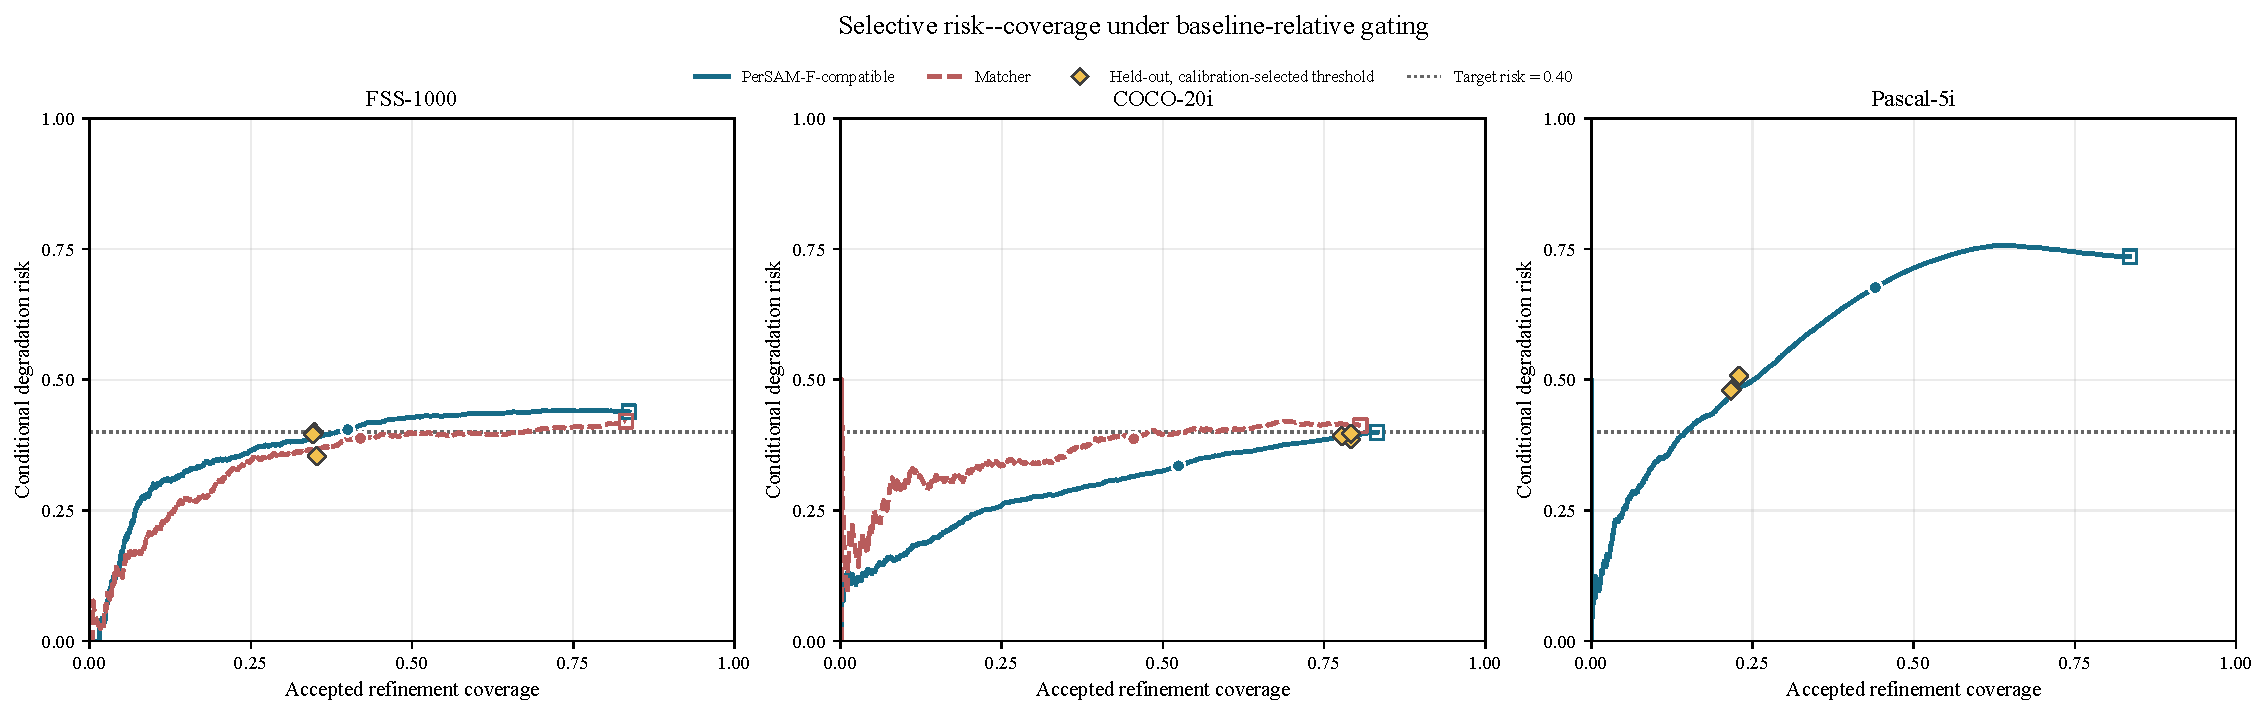
\includegraphics[width=\linewidth]{figures/generated/risk_coverage_all_generators.pdf}
\caption{Risk--coverage behavior of the baseline-relative support--foreground gate. Coverage counts accepted non-baseline refinements, while conditional degradation risk is the fraction of accepted refinements whose query mIoU is below the baseline. Solid blue curves are the PerSAM-F-compatible generator and dashed red curves are the independent Matcher generator; both curves use all available evaluation episodes. Filled circles denote the default $\lambda=0$ operating point, open squares denote the unguarded original-selector endpoint, and gold diamonds denote the three held-out evaluations at the calibration-selected threshold. The dotted horizontal line marks the empirical target risk of $0.40$. The diamonds use episode-disjoint held-out subsets and are therefore shown as operating points rather than points on the full-data curves. Query annotations are used only to evaluate the curves offline.}
\label{fig:riskcoverage}
\end{figure*}

Representative image-level cases in Fig.~\ref{fig:qualitative_rescue} complement the aggregate curves. Each row uses a different benchmark but follows the same support/query protocol. The original selector produces a lower-quality mask than the baseline, while the guarded policy rejects the proposal and returns to the baseline. These examples are qualitative illustrations; all quantitative claims use the complete evaluation sets.

\begin{figure*}[t]
\centering
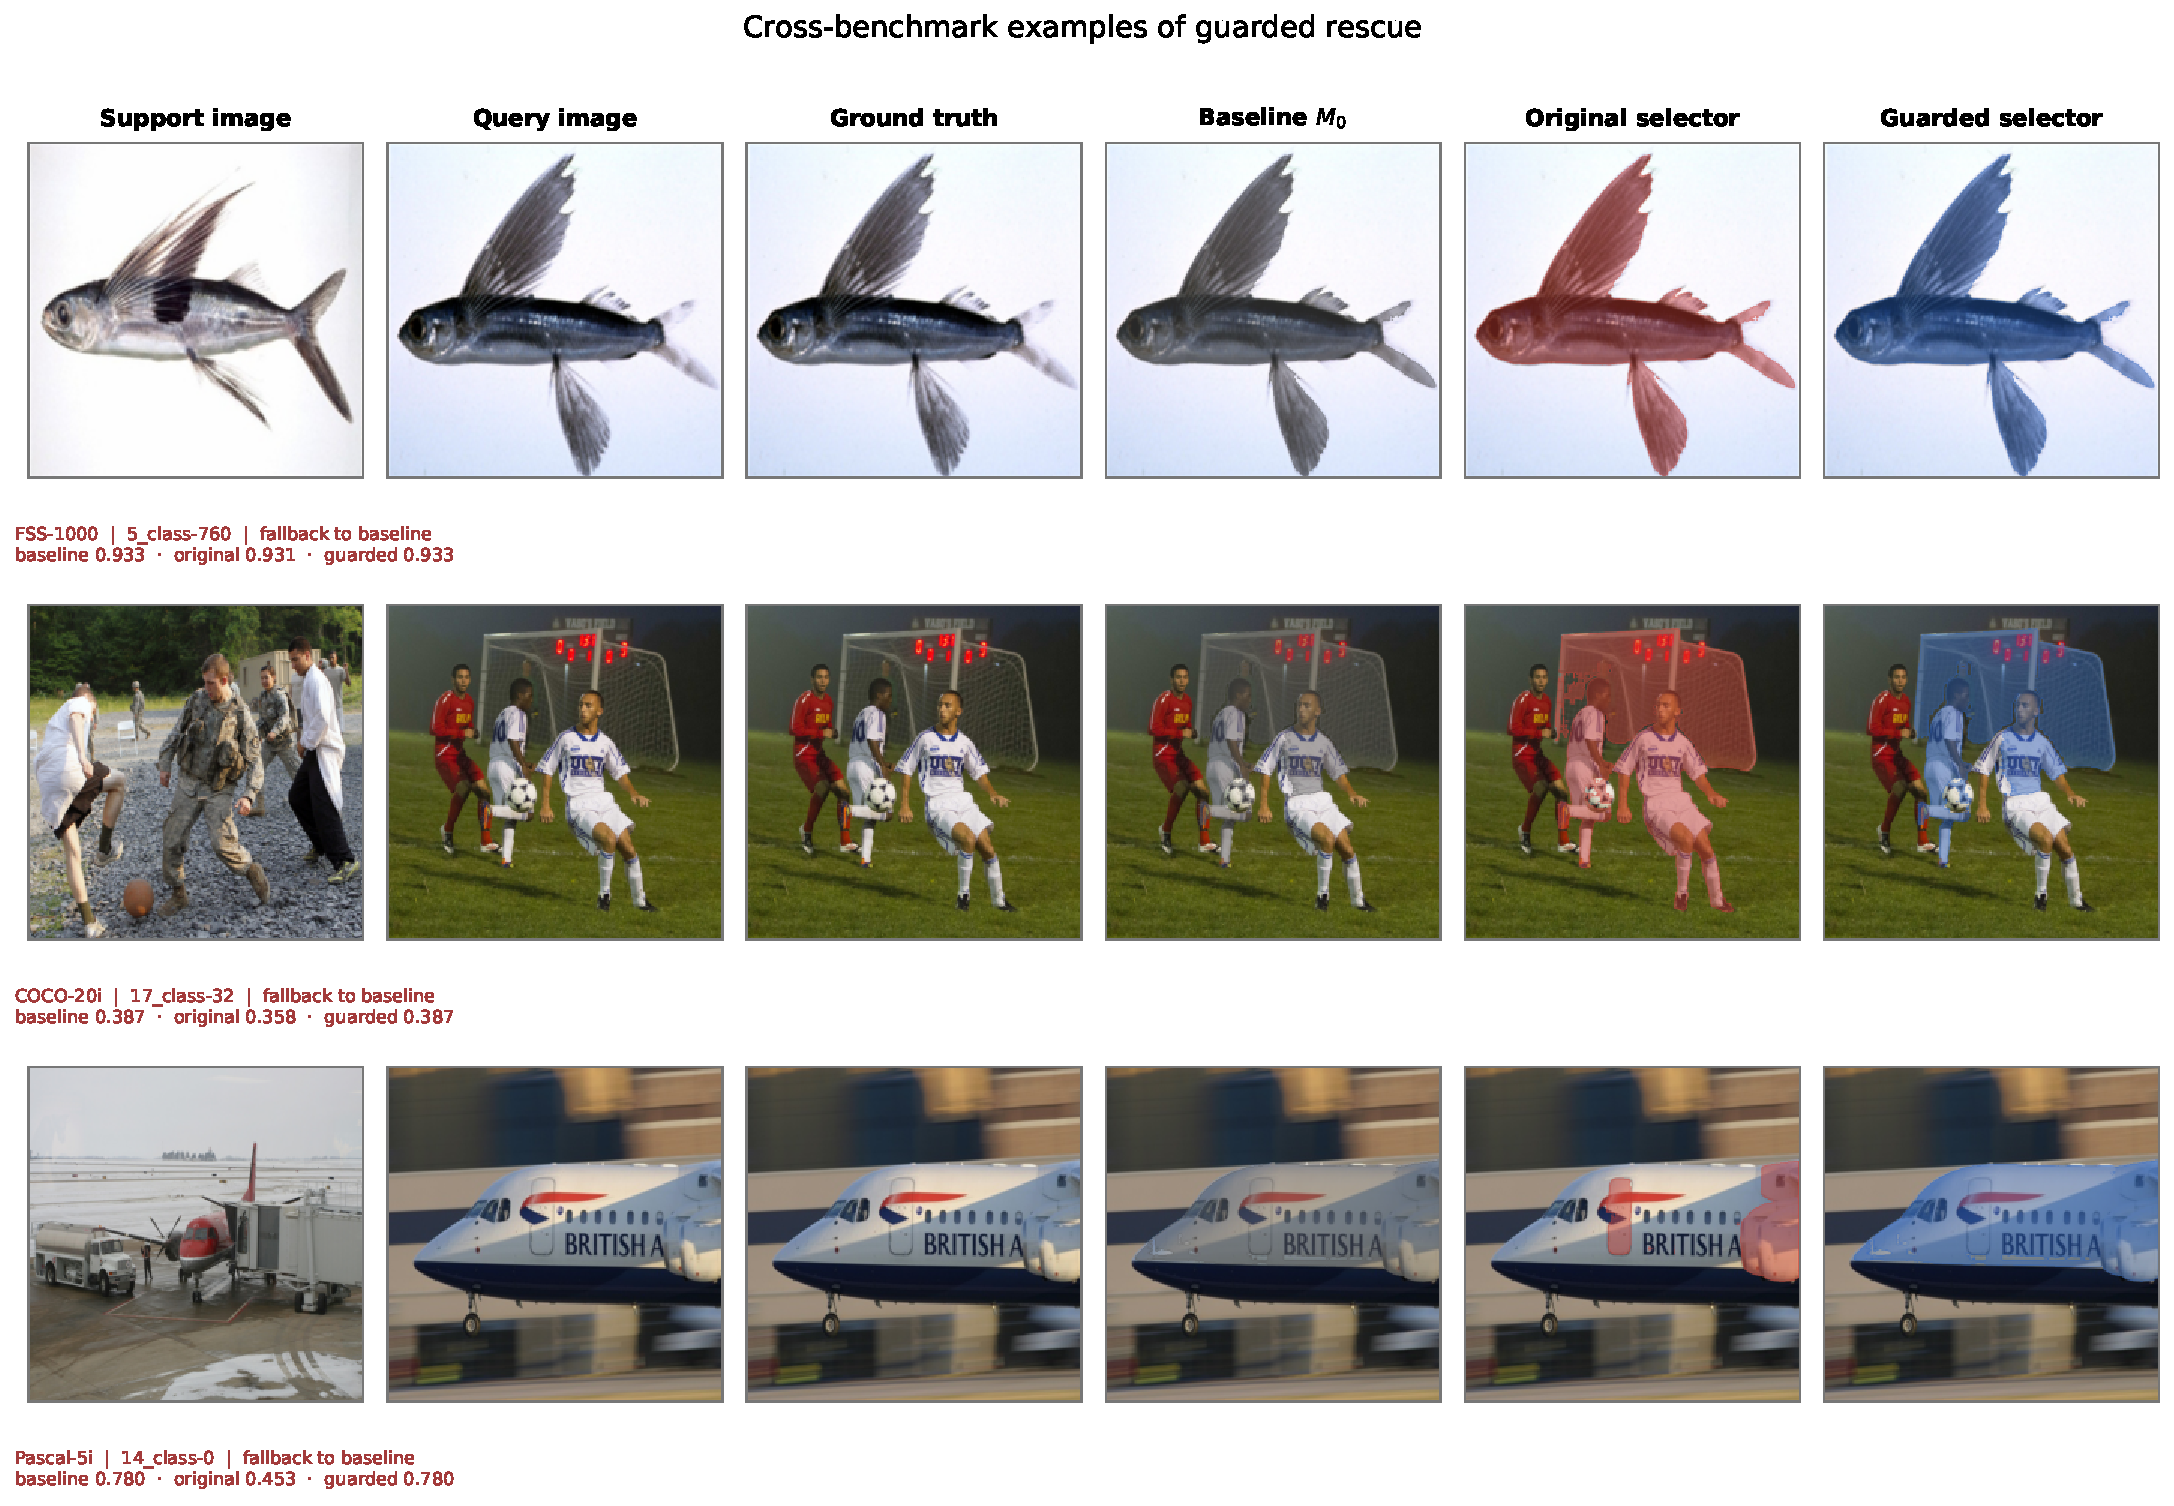
\includegraphics[width=\linewidth]{figures/generated/qualitative_cross_benchmark_rescue.pdf}
\caption{Cross-benchmark qualitative examples of guarded rescue. Each row shows a support image, a query image, the query ground truth, the baseline mask $M_0$, the original-selector output, and the guarded output. The original selector degrades relative to the baseline, while the baseline-relative gate rejects the proposal and returns to $M_0$. Green, gray, red, and blue overlays denote ground truth, baseline, original, and guarded masks, respectively.}
\label{fig:qualitative_rescue}
\end{figure*}

\subsection{Diagnostic and Boundary Analyses}

The additional diagnostics clarify how the gate changes individual decisions. Representative limitation cases (Fig.~\ref{fig:qualitative_limitations}) show that it may reject useful refinements when internal proxy signals decrease relative to the baseline. The cross-benchmark heatmap (Fig.~\ref{fig:advantage_heatmap}) separates quality gain, NDR, and gate-triggered fallback, so conservatism is not mistaken for prediction quality.

Candidate-level signal maps (Fig.~\ref{fig:signal_heatmap}) illustrate why the original proposal can differ from the oracle candidate. The transition analysis (Fig.~\ref{fig:transition_heatmap}) quantifies episode-level changes after support\_fg is applied. Rejected degraded proposals move to the non-degraded group because fallback returns the baseline. The informative question is whether these rescues preserve more mIoU than matched random rejection, as shown in Table~\ref{tab:random_control}.

\FloatBarrier

\begin{figure*}[!t]
\centering
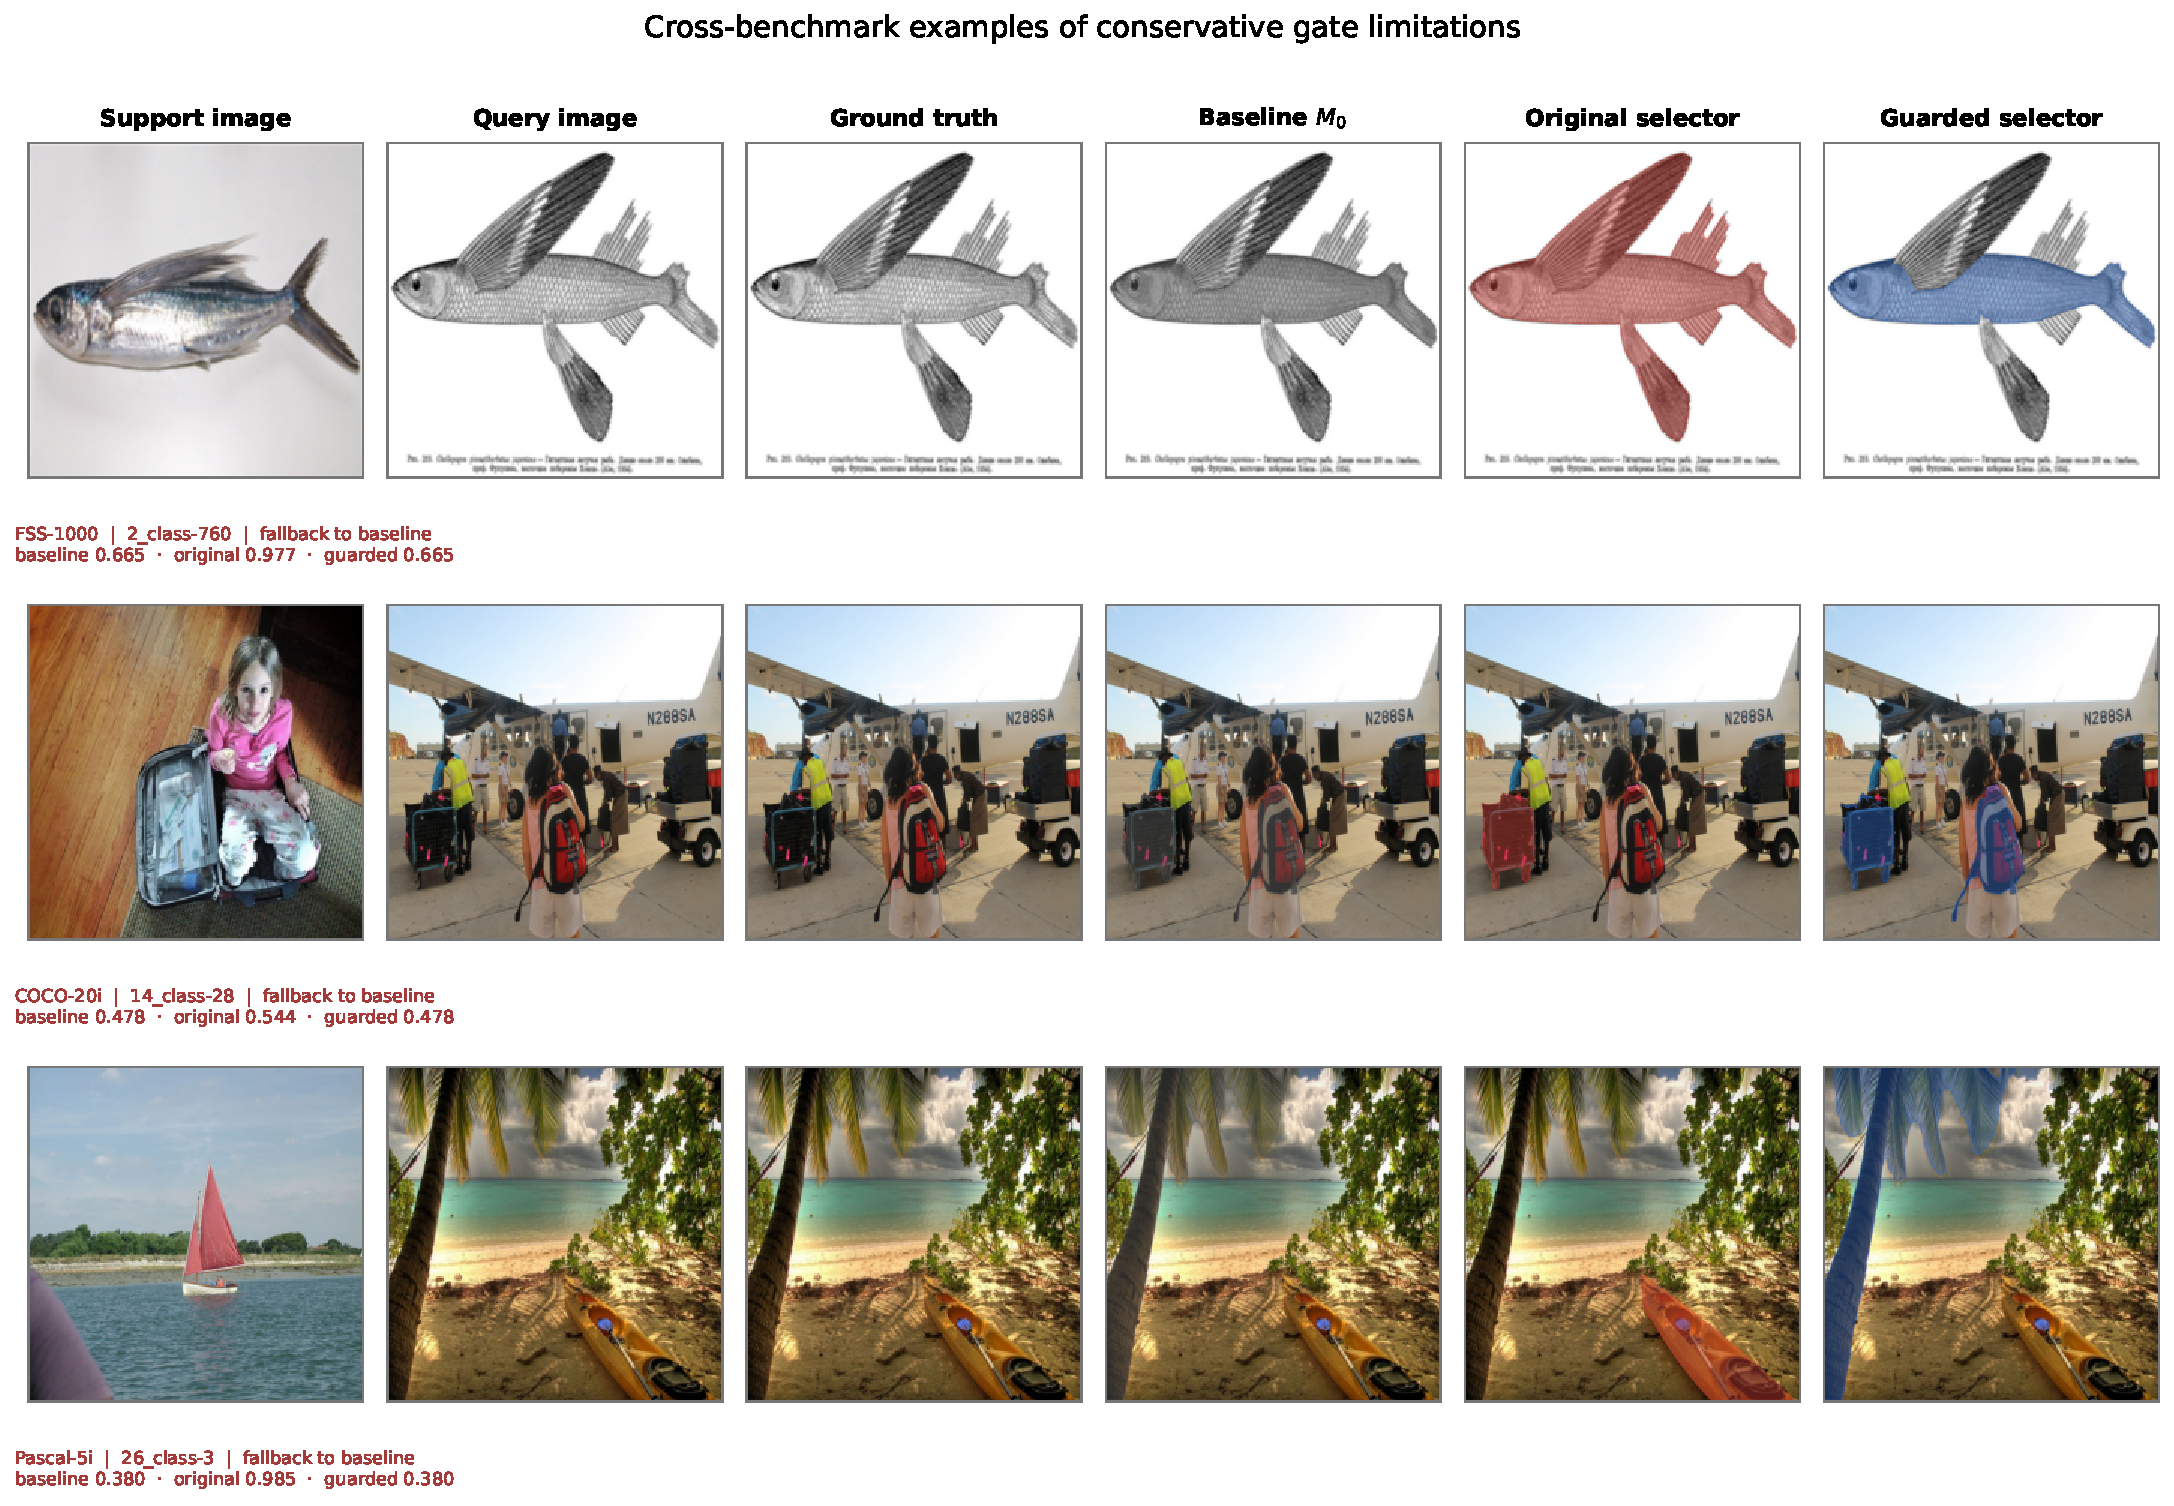
\includegraphics[width=\linewidth]{figures/generated/qualitative_cross_benchmark_limitations.pdf}
\caption{Cross-benchmark limitation cases for the conservative gate. In each row, the original selector identifies a useful refinement, but the internal baseline-relative proxy test rejects it and returns to the baseline. These examples expose the quality--safety trade-off and clarify that the gate is not a formal safety guarantee.}
\label{fig:qualitative_limitations}
\end{figure*}

\begin{figure*}[!t]
\centering
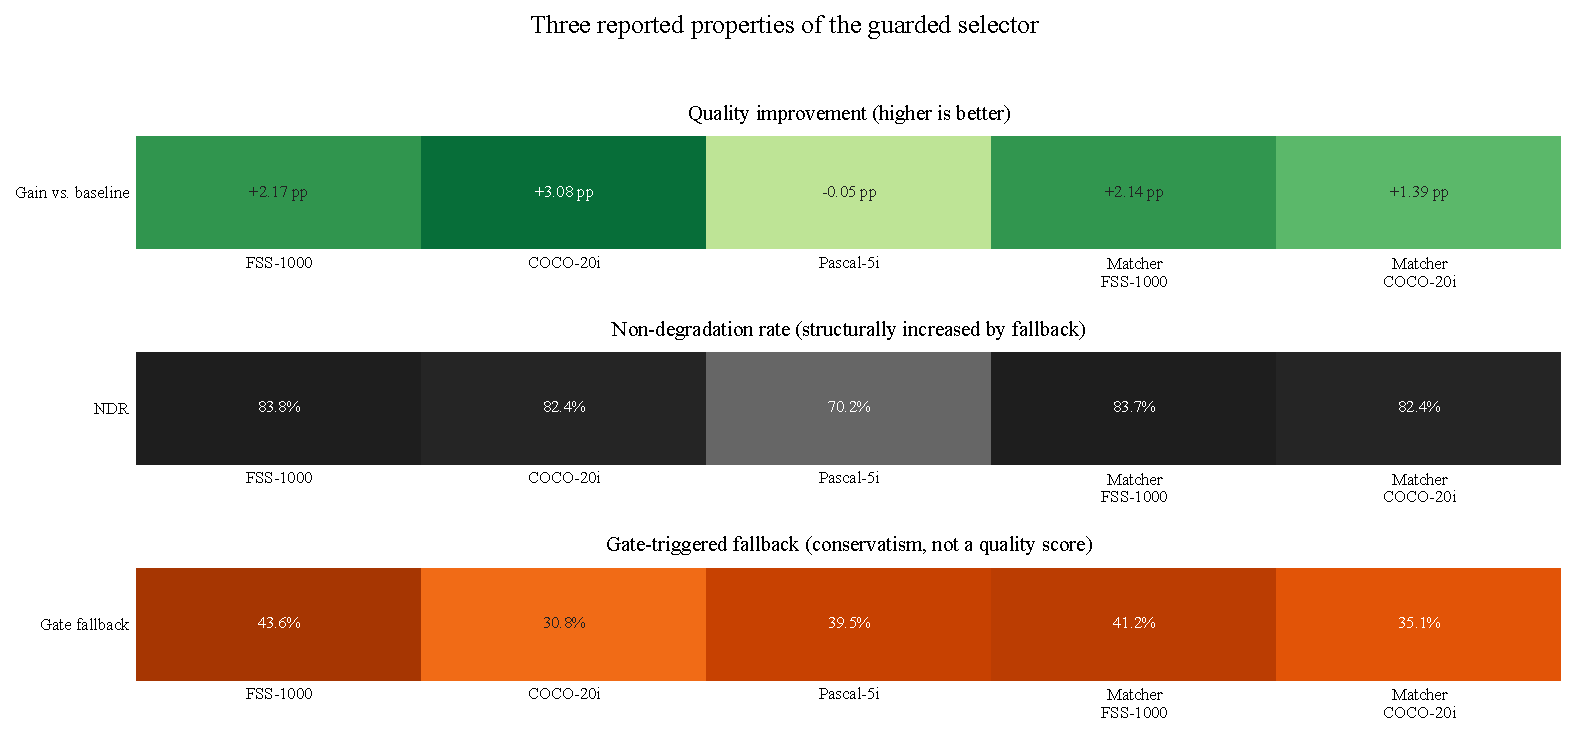
\includegraphics[width=\linewidth]{figures/generated/advantage_heatmap.pdf}
\caption{Heatmap summary of three reported properties of the guarded selector. Gain over baseline measures quality, while NDR describes baseline-relative non-degradation and increases structurally under fallback. Gate-triggered fallback measures selective conservatism rather than prediction quality.}
\label{fig:advantage_heatmap}
\end{figure*}

\begin{figure*}[!t]
\centering
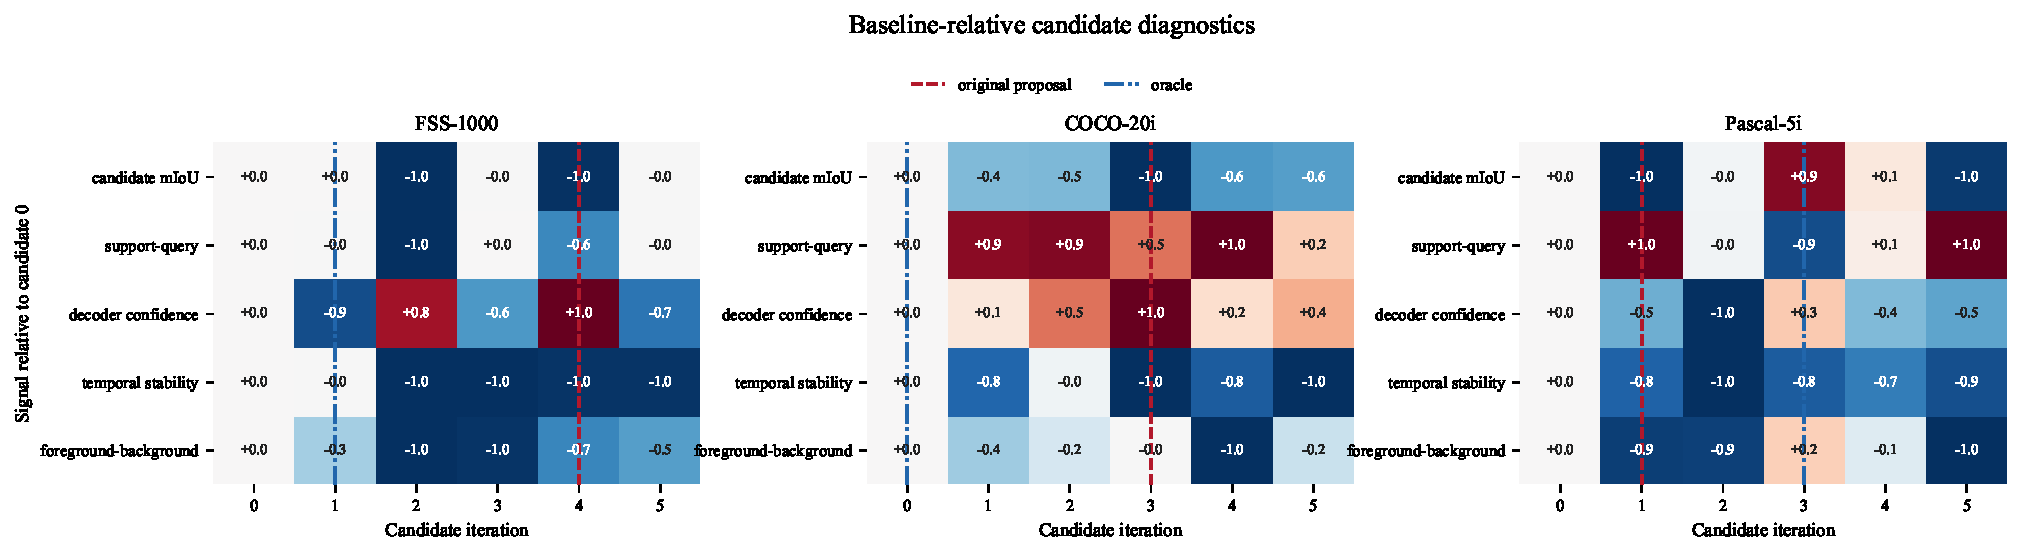
\includegraphics[width=\linewidth]{figures/generated/candidate_signal_heatmap.pdf}
\caption{Baseline-relative candidate diagnostics for representative high-regret episodes. Each panel shows candidate mIoU and the four internal signals across refinement iterations, normalized relative to candidate 0. Red dashed and blue dash-dotted lines mark the original proposal and oracle candidate, respectively.}
\label{fig:signal_heatmap}
\end{figure*}

\begin{figure*}[!t]
\centering
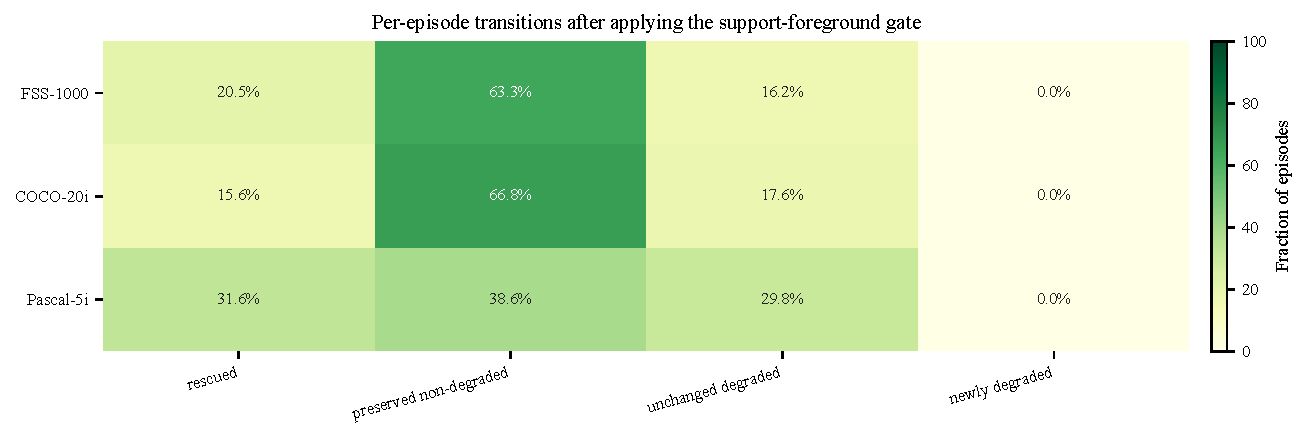
\includegraphics[width=\linewidth]{figures/generated/selection_transition_heatmap.pdf}
\caption{Per-sample transitions from the original selector to support\_fg. Rejected degraded proposals return to the baseline and therefore become non-degraded by construction. The zero newly degraded count also follows from this fallback rule and is not a separate measure of gate discrimination.}
\label{fig:transition_heatmap}
\end{figure*}

% Keep the diagnostic figures before the following Results subsection without
% forcing a sparse page break in the two-column text.
\FloatBarrier

\subsection{Comparison with Published PerSAM, Matcher, and VRP-SAM Results}

Table~\ref{tab:published} places values transcribed from the supplied published-result figures alongside our full evaluations. Some published rows use different encoders, prompts, fold aggregations, or benchmark subsets, so they provide context rather than protocol-matched comparisons.

\begin{table*}[h!t]
\center
\caption{Published external results from the supplied figures and results obtained in this study. A dash means that the supplied figure does not report that benchmark for the method. The external values are contextual comparisons, not re-runs under our exact protocol.}
\begin{tabular}{lrrrr}
\toprule
Method & FSS-1000 & COCO-20i & Pascal-5i & Source/setting \\
\midrule
PerSAM & 71.2 & 23.0 & -- & published standard FSS table \\
PerSAM-F & 75.6 & 23.5 & -- & published standard FSS table \\
PerSAM-F & 86.3 & -- & -- & alternate published FSS table \\
Matcher & 87.0 & 52.7 & -- & published standard FSS table \\
VRP-SAM (VGG-16) & -- & 48.0 & 68.7 & published one-shot table \\
VRP-SAM (ResNet-50) & -- & 53.9 & 71.9 & published one-shot table \\
Ours, Original & 88.504 & 56.564 & 65.219 & full evaluation \\
\textbf{Ours, Guarded} & \textbf{87.951} & \textbf{56.598} & \textbf{66.920} & full evaluation \\
\bottomrule
\end{tabular}
\label{tab:published}
\end{table*}

Our PerSAM-F-compatible pipeline is competitive with the reported PerSAM-F and Matcher values on FSS-1000. VRP-SAM reports higher COCO-20i and Pascal-5i values under its published settings, but its protocols are not identical to ours. Guarded PR-MaGIC addresses a different objective: limiting degradation during selection among iterative candidates. We therefore do not assign NDR, fallback, paired-selection, or oracle-gap measures to methods whose candidate pools are unavailable.

\section{Discussion}

\subsection{Why Average mIoU Is Not Sufficient}

Taken together, our results separate candidate-pool potential from selection reliability. The oracle often exceeds the baseline, showing that refinement can produce useful masks, but the original selector does not always find them. Pascal-5i makes this distinction especially clear: the selector reaches 0.652193 against a baseline of 0.669651, even though the oracle reaches 0.751492. Average candidate quality alone would hide this selection failure.

The gate turns unconstrained ranking into selective replacement. However, NDR does not establish whether the gate is informative because baseline fallback guarantees that NDR cannot decrease. An all-fallback policy would reach 100\% NDR while discarding every refinement. In practice, NDR is meaningful only when read together with mIoU, refinement coverage, and rejection-rate-matched controls.

\subsection{What the Gate Signals Capture}

Under rejection-rate matching, support\_fg exceeds random fallback by 0.42--1.17 mIoU percentage points across all five evaluations. This comparison indicates that the gate does not reject an arbitrary subset of proposals. Still, the margin provides only weak-to-moderate ranking ability, with AUROC values of 0.543--0.633. The internal signals carry useful information, but they are not calibrated estimates of segmentation quality.

\subsection{Quality--Safety Trade-off}

The gate is intentionally conservative, but the cost of that conservatism varies by benchmark. On FSS-1000, support\_fg sacrifices some mIoU relative to the original selector while rejecting proposals in 43.61\% of episodes. On COCO-20i, it preserves the original mIoU almost exactly. On Pascal-5i, frequent fallback recovers most of the original selector's loss, yet 67.63\% of accepted refinements remain degraded. When internal evidence is imperfect, no tested gate variant maximizes both quality and selectivity on every benchmark.

\subsection{Reproducibility and Scope}

All internal comparisons use the same candidate pool within each episode. The saved CSV files record candidate diagnostics, selected iteration, fallback status, mIoU, and oracle values. The complete episode-disjoint calibration output is stored in \texttt{results/multicriteria/episode\_split\_calibration.csv}. The \texttt{--selector guarded} option runs the policy online, while offline replay produces paired ablations without additional inference. Whether the same approach generalizes to non-SAM iterative systems remains an open question.

\subsection{Limitations}

The full COCO-20i and Pascal-5i experiments use three seeds across four folds, whereas FSS-1000 uses three seeds on the reported validation split. Published values may rely on different backbones, prompts, fold aggregations, or sampling procedures. The support\_fg gate is hand-designed and baseline-relative; it is neither a learned risk predictor nor a calibrated risk-control procedure. Its value also depends on the generator producing useful alternatives, and its margin discrimination is weak on FSS-1000 and Matcher. Most importantly, episode-disjoint calibration retains the 40\% empirical target on FSS-1000 and COCO-20i but misses it by 8.0--10.8 points on Pascal-5i. Larger independent calibration sets, uncertainty-aware threshold selection, distribution-shift tests, and formal risk-control methods are needed to determine whether these limits can be reduced.

\section{Conclusions}

We introduced Guarded PR-MaGIC, a training-free framework for baseline-relative candidate selection in personalized segmentation. The framework separates candidate generation from candidate acceptance and uses support consistency and foreground--background separation to decide whether a proposal should replace the baseline. Because NDR cannot decrease under this fallback construction, we evaluated gate informativeness separately. Under rejection-rate matching, guarded selection preserves more mIoU than random fallback across all five evaluations. However, the margin provides only weak-to-moderate discrimination, and accepted refinements on Pascal-5i retain high risk at the default threshold. Episode-disjoint calibration meets a 40\% empirical target on held-out FSS-1000 and COCO-20i episodes but fails on Pascal-5i, revealing a clear boundary on risk-target transfer. The transfer to Matcher further shows that the selection rule does not require retraining the candidate generator. Overall, the results support conservative candidate replacement while clearly delimiting what the internal risk signals can and cannot provide.

\appendix

\subsection*{Availability of data and materials}

The benchmark data are publicly available through the FSS-1000, COCO-20i, and Pascal-5i releases. The implementation, candidate-level analysis files, and scripts for the rejection-rate-matched control, temporal-stability ablation, and episode-disjoint calibration will be released in a public repository upon publication.

\subsection*{Author contributions}

First Author: conceptualization, methodology, software, investigation, data curation, and original-draft writing. Second Author: methodology, validation, and review and editing. Third Author: supervision, project administration, and review and editing. All authors approved the final manuscript.

\subsection*{Acknowledgements}

We thank the developers of SAM, PerSAM, Matcher, VRP-SAM, and the benchmark datasets for releasing their implementations, models, and evaluation protocols.

\subsection*{Declaration of competing interest}

The authors have no competing interests to declare that are relevant to the content of the manuscript.

\subsection*{Electronic Supplementary Material}

Supplementary material should include the full per-sample candidate tables, bootstrap outputs, temporal-stability ablation outputs, exact command configurations, and additional qualitative cases beyond those shown in the main text. The main-text diagnostic figures are generated exclusively from the saved candidate CSVs and exported masks; no external paper figures are used.

\begin{thebibliography}{99}

\bibitem{1} Kirillov, A.; Mintun, E.; Ravi, N.; Mao, H.; Rolland, C.; Gustafson, L.; Xiao, T.; Whitehead, S.; Berg, A. C.; Lo, W.-Y.; Doll{\'a}r, P.; Girshick, R. Segment Anything. In: Proceedings of the IEEE/CVF International Conference on Computer Vision, 4015--4026, 2023.

\bibitem{2} Zhang, R.; Jiang, Z.; Guo, Z.; Wu, S.; Jin, Y.; Liu, X.; Li, Y.; Zhang, S.; Zhang, P.; Gao, Z.; et al. Personalize Segment Anything Model with One Shot. In: International Conference on Learning Representations, 2024.

\bibitem{3} Shaban, A.; Bansal, S.; Liu, Z.; Essa, I.; Boots, B. One-Shot Learning for Semantic Segmentation. In: British Machine Vision Conference, 2017.

\bibitem{4} Wang, K.; Liew, J. H.; Zou, Y.; Zhou, D.; Feng, J. PANet: Few-Shot Image Semantic Segmentation with Prototype Alignment. In: Proceedings of the IEEE/CVF International Conference on Computer Vision, 9197--9206, 2019.

\bibitem{5} Min, J.; Kang, D.; Cho, M. Hypercorrelation Squeeze for Few-Shot Segmentation. In: Proceedings of the IEEE/CVF International Conference on Computer Vision, 6941--6952, 2021.

\bibitem{6} Wang, X.; Wang, Y.; Cao, L.; Huang, S.; Wang, M.; Zha, Z.-J. Painter: I/O Space Pre-training for Generalized Vision-to-Language Tasks. In: Proceedings of the IEEE/CVF Conference on Computer Vision and Pattern Recognition, 2023.

\bibitem{7} Wang, D.; Cui, J.; Wang, X.; et al. SegGPT: Segmenting Everything In Context. In: Proceedings of the IEEE/CVF International Conference on Computer Vision, 2023.

\bibitem{8} Liu, Y.; Zhu, M.; Zhang, X.; et al. Matcher: Segment Anything with One Shot Using All-Purpose Feature Matching. In: International Conference on Learning Representations, 2024.

\bibitem{9} Sun, Y.; Chen, J.; Zhang, S.; Zhang, X.; Chen, Q.; Zhang, G.; Ding, E.; Wang, J.; Li, Z. VRP-SAM: SAM with Visual Reference Prompt. In: Proceedings of the IEEE/CVF Conference on Computer Vision and Pattern Recognition, 23565--23574, 2024. DOI: 10.1109/CVPR52733.2024.02224.

\bibitem{10} Li, X.; Wei, T.; Chen, Y.; Hu, Y.; Ran, L.; Li, X. FSS-1000: A 1000-Class Dataset for Few-Shot Segmentation. In: Proceedings of the IEEE/CVF Conference on Computer Vision and Pattern Recognition, 2869--2878, 2020.

\bibitem{11} Nguyen, K.; Todorovic, S. Feature Weighting and Boosting for Few-Shot Segmentation. In: Proceedings of the IEEE/CVF International Conference on Computer Vision, 622--631, 2019.

\bibitem{12} Lee, M.; Hur, S.; Hwang, S.; Kim, W. H. PR-MaGIC: Prompt Refinement Via Mask Decoder Gradient Flow For In-Context Segmentation. In: Proceedings of the IEEE/CVF Conference on Computer Vision and Pattern Recognition, 2026.

\bibitem{13} El-Yaniv, R.; Wiener, Y. On the Foundations of Noise-Free Selective Classification. Journal of Machine Learning Research, 11(53), 1605--1641, 2010.

\bibitem{14} Geifman, Y.; El-Yaniv, R. Selective Classification for Deep Neural Networks. In: Advances in Neural Information Processing Systems, Vol. 30, 2017.

\bibitem{15} Bates, S.; Angelopoulos, A.; Lei, L.; Malik, J.; Jordan, M. I. Distribution-Free, Risk-Controlling Prediction Sets. Journal of the ACM, 68(6), 1--34, 2021. DOI: 10.1145/3478535.

\end{thebibliography}

% for bibtex
% \bibliographystyle{CVMbib}
% \bibliography{refs}

\subsection*{Author biography}
\note{(Replace the following placeholders with the required photographs and biographies before submission.)}

\begin{biography}[author1]{First Author} Please supply the author's photograph and a one-paragraph biography describing study experience, research interests, and awards received.\end{biography}

\end{document}
